\vspace{-0.1\baselineskip}
\section{Experiments}
\vspace{-0.1\baselineskip}
\label{sec:experiments}
We perform all experiments using our collected dataset, and evaluate multiple system settings for pose and segment to validate each component.
For obtaining GPS and IMU signal, due to at each time step, only one sampled noisy signal can obtained. This is limited for training the system. Thus, follow~\cite{vishal2015accurate}, we simulate noisy GPS and IMU by adding random perturbation $\epsilon$ \wrt ground truth pose following uniform distributions. 
Specifically, translation and rotation noise are set as $\epsilon_t \sim U(0, 7.5m)$ and $\epsilon_r \sim U(0^{\circ}, 15^{\circ})$ respectively. 
We refer to realistic data~\cite{lee2015gps} for setting the noisy range of simulation.

In this paper, our data vehicle collected 6 videos at different daytimes surrounding a technology park. The 3D map generated in our experiment has a road length around 3500$m$, and the distance between consecutive frames is around 5$m$ to 10$m$. We use 4 of the videos for training and 2 for testing, yielding 2242 training images and 756 testing images. The semantic classes, as shown in \figref{fig:data}, include $\{$sky, car-lane, pedestrian-lane, bike-lane, curb, traffic-cone, traffic-stack, traffic-fence, light-pole, traffic-light, tele-pole, traffic-sign, billboard, building, security-stand, plants, object $\}$. In the future, we are targeting at constructing even larger datasets with more semantics.

\textbf{Implementation details.} To quickly render from the 3D map, we adopt OpenGL to efficiently render a label map with the z-buffer handling. A 512 $\times$ 608 image can be generated in 70ms with a single Titan Z GPU, which is also the input size for both pose CNN and segment CNN. 
For pose CNN, the filter size of each layers is $\{32, 32, 64, 128, 256, 1024, 128, 7\}$, and the forward speed for each frame is 9ms. For pose RNN, we sample sequences with length of 100 from our data for training, and on average is cost 0.9ms for each frame.
For segment CNN, we keep the size the same as input, and the forward times is 90ms. 
Both of the network is learned with 'Nadam' optimizer~\cite{dozat2016incorporating} with a learning rate $10^{-3}$. We sequentially train the three models due to GPU memory limitation.
Specifically, for pose CNN and segment CNN, we stops at 150 epochs when there is no performance gain, and for pose RNN, we stops at 200 epochs. For data augmentation, we use the imgaug\footnote{https://github.com/aleju/imgaug} library to variate lighting, blurring and flipping. We select a subset from training images for validating the trained model from each epoch, and choose the model performing best for evaluation.

For testing, since input GPS/IMU contains variations, \ie~$\ve{p}_t^c=\ve{p}^*+\epsilon$, we need to have a confidence range of prediction for both camera pose and image segment, in order to verify the improvement of each component we have is significant. Specifically, we report the standard variation of the results from a 10 time simulation to obtain the confidence range. Finally, we implement all the networks by adopting the MXNet~\cite{ChenLLLWWXXZZ15} platform.

For pose evaluation, we use the median translation offset and median relative angle~\cite{Kendall_2015_ICCV}. For evaluating segment, we adopt the commonly use pixel accuracy (Pix. Acc.), mean class accuracy (mAcc.) and mean intersect-over-union (mIOU) as that from~\cite{WuSH16e}.

\begin{table}
\vspace{-0\baselineskip}
\center
\fontsize{7}{8}\selectfont
\hspace*{-0.33cm}
\begin{tabular}{llll}
\toprule[0.1 em]
% \thickhline
Method & Trans (m) $\downarrow$ & Rot ($\circ$)$\downarrow$  & Pix. Acc($\%$)$\uparrow$ \\
\hline
PoseNet~\cite{kendall2017geometric} & -  & -  & -  \\
Noisy pose & 3.45 $\pm$ 0.176 & 7.87 $\pm$ 1.10 & 54.01 $\pm$ 1.5 \\
Pose CNN w/o semantic & 1.355 $\pm$ 0.052  & 0.982 $\pm$ 0.023 & 70.99 $\pm$ 0.18 \\
Pose CNN w semantic & 1.331 $\pm$ 0.057  & 0.727 $\pm$ 0.018 & 71.73 $\pm$ 0.18  \\
Pose RNN w/o CNN & 1.282 $\pm$ 0.061  & 1.731 $\pm$ 0.06 &  68.10 $\pm$ 0.32 \\
Pose CNN w KF & 1.281 $\pm$ 0.06  & 0.833 $\pm$ 0.03 & 72.00 $\pm$ 0.17  \\
Pose CNN-RNN  & \textbf{1.005} $\pm$ 0.044  & \textbf{0.719} $\pm$ 0.035  & \textbf{73.01} $\pm$ 0.16  \\
\toprule[0.1 em]
\end{tabular}
\caption{Compare the accuracy of different settings for pose estimation.
Noisy pose indicates the noisy input signal from GPS, IMU, and 'KF' means kalman filter.
The number after $\pm$ indicates the std from 10 simulations. $\downarrow \& \uparrow$ means lower the better and higher the better respectively. 
We can see the improvement is statistically significant.}
\label{tbl:pose}
\vspace{-1.5\baselineskip}
\end{table}

\textbf{Pose Evaluation.}
In \tabref{tbl:pose}, we show the performance of estimated translation $\ve{t}$ and rotation $\ve{r}$ from different model variations. We first directly follow the work of PoseNet~\cite{Kendall_2015_ICCV,kendall2017geometric}, and use their published code and geometric loss (\equref{eq:proj_loss}) to train a model. 
Due to scene appearance similarity of the street-view, we did not obtain a reasonable model, \ie~results better than the noisy GPS/IMU signal.
At the 2nd row, we show the median error of GPS and IMU from our simulation. 
At the 3rd row, by using our pose CNN, the model can learn good relative pose between camera and GPS/IMU, which significantly reduces the error (60$\%$ for $\ve{t}$, 85$\%$ for $\ve{r})$. 
By adding semantic cues, \ie road priori and semantic weights in \equref{eq:proj_loss}, the pose errors are further reduced, especially for rotation (from $0.982$ to $0.727$ at the 4th row). Actually, we found the most improvement is from semantic weighting, while the road priori helps marginally in this experiment so we drop the numbers. However, in the future, we would like to experiment larger noise and more data variations, which will better validate different cues.

For evaluating an video input, we setup a baseline of performing RNN directly on the GPS/IMU signal, and as shown at 'Pose RNN w/o CNN', the estimated $\ve{t}$ is even better than pose CNN, while $\ve{r}$ is comparably much worse. This meets our expectation since the speed of camera is easier to capture temporally than rotation. Another baseline we adopt is performing Kalman filter~\cite{kalman1960new} to the output from Pose CNN by assuming a constant speed which we set as the averaged speed from training sequences. As shown at 'Pose CNN w KF', it does improve slightly for translation, but harms rotation, which means the filter over smoothed the sequence. Finally when combining pose CNN and RNN, it achieves the best pose estimation both for $\ve{t}$ and $\ve{r}$.

% Finally, RNN gives strong cues about the moving speed and acceleration of the camera, yields the best results for both translation and rotation.
\begin{figure*}
\center
\vspace{-0.3\baselineskip}
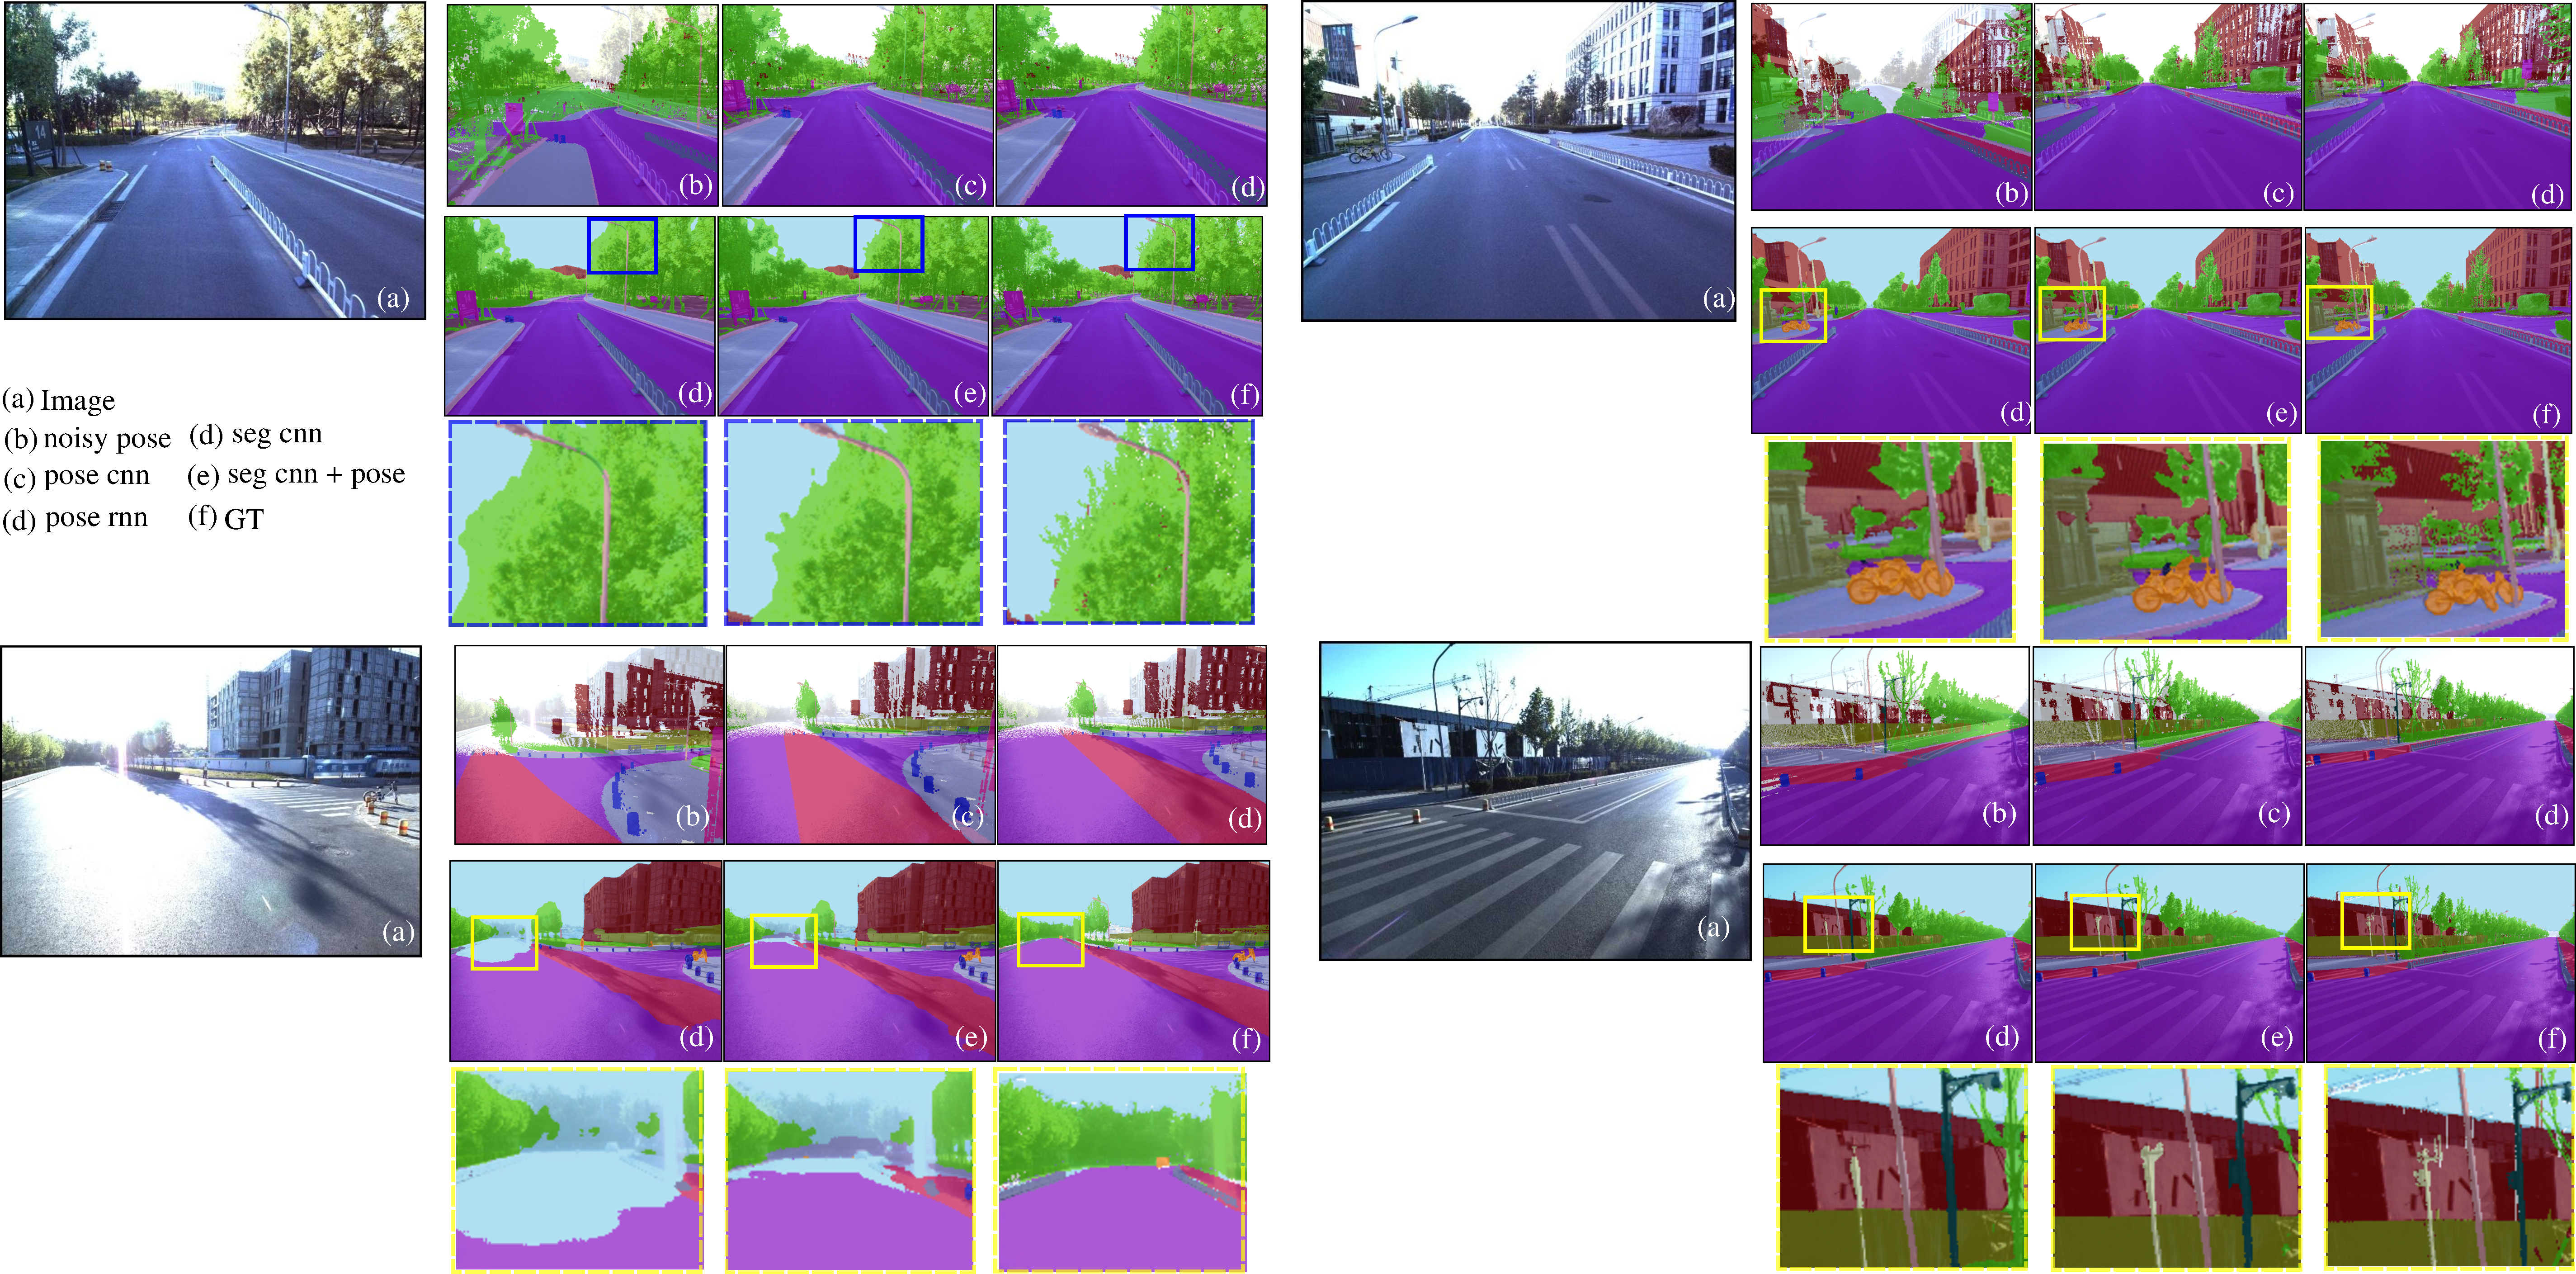
\includegraphics[width=0.99\textwidth]{fig/results.pdf}
   \caption{Results from each intermediate stage out of the system. The meaning of each label map (b-g) for an image (a) is indicated by a layout map at left top. Improved regions are boxed and zoomed out for visualization (best in color).}
\label{fig:results}
\vspace{-1.2\baselineskip}
\end{figure*}

\begin{table*}[!htbp]
\center
\fontsize{6}{6}\selectfont
\setlength\tabcolsep{1.5pt}
\begin{tabular}{lccccccccccccccccccccc}
% \toprule[0.1 em]
%\thickhline
Method & \rot{mIOU} & \rot{mAcc} & \rot{Pix. Acc}   & \rot{sky} & \rot{car-lane} & \rot{ped-lane} & \rot{bike-lane} & \rot{curb} & \rot{$t$-cone} & \rot{$t$-stack} & \rot{$t$-fence} & \rot{light-pole} & \rot{$t$-light} & \rot{tele-pole} & \rot{$t$-sign} & \rot{billboard} & \rot{temp-build} & \rot{building} & \rot{sec.-stand} & \rot{plants} & \rot{object} \\
\hline
ResNet38~\cite{WuSH16e}                      &64.66  &71.92 & 95.87 &93.6 &98.5 &82.9 &87.2 &61.8 &46.1 &41.7 &82.0 &37.5 &26.7 &45.9 &49.5 &60.0 &85.1 &67.3 &38.0 &89.2 &66.3\\
SegCNN w/o Pose                              &68.35  &77.09 & 95.61 &94.2 &98.6 &83.8 &89.5 &69.3 &47.5 &52.9 &83.9 &52.2 &43.5 &46.3 &52.9 &66.9 &87.0 &69.2 &40.0 &88.6 &63.8 \\
SegCNN w pose GT                             &79.37  &86.8  & 97.1  &96.1 &99.4 &92.5 &93.9 &81.4 &68.8 &71.4 &90.8 &71.7 &64.2 &69.1 &72.2 &83.7 &91.3 &76.2 &58.9 &91.6 &56.7 \\
SegCNN w Pose CNN &68.6$\pm$0.12 & 77.95$\pm$0.16 & 95.67$\pm$0.01  &94.5 &98.7 &84.3 &89.3 &69.0 &46.8 &52.9 &84.9 &53.7 &39.5 &48.8 &50.4 &67.9 &87.5 &69.9 &42.8 &88.5 &60.9 \\
SegCNN Final    &\textbf{69.93}$\pm$0.08  & \textbf{79.36}$\pm$0.08 &\textbf{95.98}$\pm$0.004 &
                                             94.9 &98.8 &85.3 &90.2 &71.9 &45.7 &57.0 &85.9 &58.5 &41.8 &51.0 &52.2 &69.4 &88.5 &70.9 &48.0 &89.3 &59.5 \\
\toprule[0.1 em]
\vspace{-1.0\baselineskip}
\end{tabular}
\caption{Compare the accuracy of different segment networks setting. $t$ is short for 'traffic' in the table. $\pm$ indicates the confidence region by 10 times simulation, which we drop for per-class accuracy. Our results are especially good at parsing of detailed structures and scene layouts, which is visualized in~\figref{fig:results}.}
\label{tbl:segment}
\vspace{-1.8\baselineskip}
\end{table*}


\textbf{Segment Evaluation.}
In \tabref{tbl:segment}, we show the scene parsing results. 
Firstly, we adopt one of the SOTA parsing network on the CityScapes, \ie~ResNet38~\cite{WuSH16e}, and train it with our data. It has pre-trained parameters from the ImageNet~\cite{deng2009imagenet} dataset, and run with a 1.03$s$ per-frame with our resolution. As shown at the 1st row, it achieve reasonable accuracy compare to our segment CNN (2nd row) when there is no pose priori. However, our network is 10x faster, and runs in 90ms. 
At 3rd row, we use the ground truth pose rendered label map as segment CNN priori to obtain an upper-bound for the segmentation performance. 
In this case, the rendered label map aligns perfect with the image, thus yields significantly better results without miss classify most of the static background.
% At 4th row, we train the segment network without pose prior.  
% Notice that for a fair comparison, after convergence at 100 epoch, we continue train the network another 100 epochs in order to avoid the influence from longer training.
At 4th and 5th row, we show the results trained with rendered label map from pose CNN and pose CNN-RNN respectively. We can see using pose CNN, the results just improve slightly compare to the segment CNN, from our observation, this is because the offset is still significant for some detailed structures, \eg light-pole.
However, when using the pose after RNN, better alignment is achieved and the segment accuracy improves significantly especially for thin structured regions like pole, as visualized in~\figref{fig:results}, which demonstrates the effectiveness of our strategy. 
Here, we leave per-class results to the supplementary materials as space limitation.


% \begin{table}[b]
% \vspace{-1.0\baselineskip}
% \center
% \hspace*{-0.3cm}
% \fontsize{8}{8}\selectfont
% \begin{tabular}{lccc}
% \toprule[0.1 em]
% %\thickhline
% Method & mIOU($\%$) $\uparrow$ &  mAcc($\%$) $\uparrow$& Pix. Acc($\%$) $\uparrow$ \\
% \hline
% ResNet38~\cite{WuSH16e} &64.66  & 71.92 & 95.87  \\
% SegCNN w/o Pose & 68.35 & 77.09 & 95.61 \\
% SegCNN w pose GT &79.37  & 86.8 & 97.1 \\
% % SegCNN $\xi$ Pose & 95.63 $\pm$ 0.02 & 77.39 $\pm$ 0.21 & 68.41 $\pm$ 0.15\\
% SegCNN w Pose CNN &68.6 $\pm$ 0.12 & 77.95 $\pm$ 0.16 & 95.67 $\pm$ 0.01 \\
% SegCNN Final & \textbf{69.93} $\pm$ 0.08  & \textbf{79.36} $\pm$ 0.08 &\textbf{95.98} $\pm$ 0.004 \\
% \toprule[0.1 em]
% \end{tabular}
% \caption{Compare the accuracy of different network settings. $\pm$ indicates the standard variation by 10 times GPS simulation. 
% Full table for all class accuracy is available in our supplementary materials.}
% \label{tbl:segment}
% \vspace{-1.3\baselineskip}
% \end{table}

In \figref{fig:results}, we visualize several examples from our dataset. In the figure, we can see the noisy pose (b), is progressively rectified by pose CNN (c) and pose RNN (d) from view of camera. Additionally, at (e) and (f), we compare the segment results without and with camera pose respectively. As can be seen at the boxed regions, the segment results with pose rendered label maps do provide better accuracy in terms of capturing region details at the boundary, discovering rare classes and keeping correct scene layout. All of above could be important for navigation, \eg figuring out the traffic signs and tele-poles that are visually hard to detect.
